\typeout{(body.tex)}

\begin{frame}
    \titlepage
\end{frame}

% asymptotic growth rates
\begin{frame}{asymptotic growth rate or \textit{order}}
\begin{itemize}
\item compare two functions, but\ldots
\item ignore constant factors, small inputs
\item<2-> example: {\color{red!70!black}$f(n) = 1\,000\,000 \cdot n^2$}; {\color{blue!70!black}$g(n) = 2^n$}
    \begin{itemize}
    \item $g$ grows faster --- eventually much bigger than $f$
    \end{itemize}
\end{itemize}
\begin{tikzpicture}
\begin{visibleenv}<3->
\begin{axis}[width=12.5cm,height=5.5cm,samples=50,xmin=1,xmax=35,ymin=0,ymax=2e9]
\addplot[draw=red,very thick,domain=1:35] {1000000*x^2};
\addplot[draw=blue,very thick,domain=1:31] {2^x};
\begin{visibleenv}<4->
\fill[green,opacity=0.05] (axis cs:30,0) rectangle (axis cs:35,2147483648);
\draw[thick,-Latex] (axis cs:25,1.5e9) node[left] {goal: predict behavior here} -- (axis cs:31,1.5e9);
\end{visibleenv}
\begin{visibleenv}<5->
\fill[red,opacity=0.05] (axis cs:1,0) rectangle (axis cs:27,0.75e9);
\draw[thick,-Latex] (axis cs:10,0.8e9) node[above,inner sep=0.5mm] {ignore behavior here} -- (axis cs:10,0.5e9);
\end{visibleenv}
\end{axis}
\end{visibleenv}
\end{tikzpicture}
\end{frame}

\begin{frame}{preview: what functions?}
\begin{itemize}
    \item example: comparing sorting algorithms
    \item $\text{runtime} = f(\text{size of input})$
        \begin{itemize}
        \item e.g. $\text{seconds to sort} = f(\text{number of elements in list})$
        \item e.g. $\text{\# operations to sort} = f(\text{number of elements in list})$
        \end{itemize}
    \item $\text{space} = f(\text{size of input})$
        \begin{itemize}
        \item e.g. $\text{number of bytes of memory} = f(\text{number of elements in list})$
        \end{itemize}
\end{itemize}
\end{frame}

\begin{frame}{theory, not empirical}
    \begin{itemize}
    \item yes, you can make \textit{guesses} about big-oh behavior from measurements
    \item but, no, graphs $\not=$ big-oh comparison
    \begin{itemize}
        \item what happens further to the right?
        \item might not have tested big enough
    \end{itemize}
    \vspace{.5cm}
    \item want to write down \myemph{formula}
    \item<2-> example: summing a list of $n$ items:
        \begin{itemize}
        \item exactly $n$ addition operations
        \item \textit{assume} each one takes $k$ unit of time
        \item $\text{runtime} = f(n) = kn$
        \end{itemize}
    \end{itemize}
\end{frame}


% why asymptotic
    % big inputs
    % from course introduction slides
\begin{frame}{recall: comparing list data structures}
\begin{itemize}
    \item List benchmark (from intro slides) w/ 100000 elements
\end{itemize}
\begin{tabular}{lr@{.}lr@{.}lr@{.}lr@{.}l}
Data structure & \multicolumn{2}{c}{Total}  & \multicolumn{2}{c}{Insert}& \multicolumn{2}{c}{Search} & \multicolumn{2}{c}{Delete}  \\
    {\tt Vector} &  \myemph<2>{87} & \myemph<2>{818} & 0 & 004 & \myemph<2,5>{63} & \myemph<2,5>{202} & \myemph<2,5>{24} & \myemph<2,5>{612} s \\
    {\tt ArrayList} & \myemph<2>{87} & \myemph<2>{192} & 0 & 010 & \myemph<2,5>{62} & \myemph<2,5>{470} & \myemph<2,5>{24} & \myemph<2,5>{712} s\\
    {\tt LinkedList} & \myemph<2>{263} & \myemph<2>{776} & 0 & 006 & \myemph<2,5>{196} & \myemph<2,5>{550} & \myemph<2,5>{67} & \myemph<2,5>{439} s\\
    {\tt HashSet} & \myemph<3>{0} & \myemph<3>{029} & 0 & 022 & \myemph<6>{0} & \myemph<6>{003} & \myemph<6>{0} & \myemph<6>{004} s\\
{\tt TreeSet} & \myemph<3>{0} & \myemph<3>{134} & 0 & 110 & 0 & 017 & 0 & 007 s\\
{\tt Vector}, sorted &  2 & 642 & 0 & 009 & 0 & 024 & 2 & 609 s\\
\end{tabular}
\begin{tikzpicture}[overlay,remember picture]
\coordinate (place) at ([yshift=.5cm]current page.south);
\tikzset{
    box/.style={anchor=south,at={(place)},align=left,draw=red,thick}
}
\begin{visibleenv}<2>
\node[box] {some runtimes get really big as size gets large\ldots};
\end{visibleenv}
\begin{visibleenv}<3>
    \node[box] {others seem to remain manageable};
\end{visibleenv}
\begin{visibleenv}<4>
    \node[box] {problem: \myemph{growth rate} of runtimes with list size};
\end{visibleenv}
\begin{visibleenv}<5>
    \node[box] {
        for {\tt Vector} (unsorted), {\tt ArrayList}, {\tt LinkedList}\ldots \\
        \# operations grows like $n$ where $n$ is list size
    };
\end{visibleenv}
\begin{visibleenv}<6>
    \node[box] {
        for {\tt HashSet}\ldots \\
        \# operations per search/remove is constant (sort of)
    };
\end{visibleenv}
\begin{visibleenv}<7>
    \node[box] {
        for {\tt TreeSet}, sorted {\tt Vector}\ldots \\
        \# operations per search grows like $\log(n)$ where $n$ is list size
    };
\end{visibleenv}
\end{tikzpicture}
\end{frame}

\begin{frame}{why asymptotic analysis?}
    \begin{itemize}
    \item ``can my program work when data gets big?''
        \begin{itemize}
        \item website gets thousands of new users?
        \item text editor opening 1MB book? 1 GB log file?
        \item music player sees $1\,000$ song collection? $50\,000$?
        \item text search on 100 petabyte copy of the text of the web?
        \end{itemize}
    \item<2-> if asymptotic analysis says ``no''
        \begin{itemize}
            \item can find out \myemph{before implementing algorithm}
            \item won't be fixed by, e.g., buying a faster CPU
        \end{itemize}
    \end{itemize}
\end{frame}


% big-omega, big-theta, big-oh 
    % + Venn diagram
    % FIXME: Venn diagram
\begin{frame}{sets of functions}
\begin{itemize}
\item define sets of functions based on an example $f$
\vspace{.5cm}
\item $\Omega(f)$: grow no slower than $f$ (``$\ge f$'')
\item $O(f)$: grow no faster than $f$ (``$\le f$'')
\item $\Theta(f) = \Omega(f) \cap O(f)$: grow as fast as $f$ (``$= f$'')
\vspace{.5cm}
\item<2-> examples:
    \begin{itemize}
        \item $n^3 \in \Omega(n^2)$ 
        \item $100n \in O(n^2)$ 
        \item $10n^2+n \in \Theta(n^2)$ --- ignore constant factor, etc.
            \begin{itemize}
            \item and $10n^2+n \in O(n^2)$ and $10n^2+n \in \Omega(n^2)$
            \end{itemize}
    \end{itemize}
\end{itemize}
\end{frame}


% time complexity assumptions
    % measured with input sizes
    % comparing *functions*
    % comparing *worst-cases*
\begin{frame}{what are we measuring}
\begin{eqnarray*}
    f(n) &=& \text{\myemph<3>{worst case} running time} \\
    n    &=& \text{input size --- as a positive integer} \\
\end{eqnarray*}
    \begin{itemize}
        \item<2-> will comapre $f$ to another function $g(n)$
        \item<2-> example: $f(n) \in O(g(n))$ (or $f \in O(g)$)
            \begin{itemize}
                \item informally: ``$f$ is big-oh of $g$''
            \end{itemize}
        \item<2-> example $f(n) \not\in \Omega(g(n))$ or ($g \not\in \Omega(g)$)
            \begin{itemize}
            \item informally: ``$f$` is not big-omega of $g$''
            \end{itemize}
    \end{itemize}
\end{frame}

\begin{frame}{worst case?}
    \begin{itemize}
    \item this class: almost always \myemph{worst cases}
    \item intuition: detect if program will \textit{ever} take ``forever''
    \vspace{.5cm}
    \item<2-> example: iterating through an array until we find a value
        \begin{itemize}
        \item best case: look at one value, it's the one we want
        \item worst case: look at every value, none of them are what we want
        \end{itemize}
    \end{itemize}
\end{frame}


% formal definitions
% examples of formal definition
    % O
\begin{frame}{formal definitions}
    \begin{itemize}
    \item $f(n) \in O(g(n))$ if and only if \\
        \hspace{.5cm}there exists $c > 0$ and $n_0 > 0$ such that \\
            \hspace{.5cm}$f(n) \le c \cdot g(n)$ for all $n > n_0$
    \item $f(n) \in \Omega(g(n))$ if and only if \\
        \hspace{.5cm}there exists $c > 0$ and $n_0 > 0$ such that \\
        \hspace{.5cm}$f(n) \le c \cdot g(n)$ for all $n > n_0$
    \item $f(n) \in \Theta(g(n))$ if and only if \\
          $f(n) \in O(g(n))$ and $f(n) \in \Omega(g(n))$
    \end{itemize}
\end{frame}

\begin{frame}{formal definition example (1)}
    \begin{itemize}
    \item $f(n) \in O(g(n))$ if and only if \\
        \hspace{.5cm}there exists $c > 0$ and $n_0 > 0$ such that \\
        \hspace{.5cm}$f(n) \le c \cdot g(n)$ for all $n > n_0$
    \item Is $ n \in O(n^2)$:
        \begin{itemize}
        \item<2-> choose $c = 1$, $n_0 = 2$
        \item<2-> for $n > 2=n_0$: $n \le c\cdot n^2 = n^2$
        \item<2-> Yes!
        \end{itemize}
    \end{itemize}
\end{frame}

\begin{frame}{formal definition example (2)}
    \begin{itemize}
    \item $f(n) \in O(g(n))$ if and only if \\
        \hspace{.5cm}there exists $c > 0$ and $n_0 > 0$ such that \\
        \hspace{.5cm}$f(n) \le c \cdot g(n)$ for all $n > n_0$
    \item Is $10n \in O(n)$?
        \begin{itemize}
        \item<2-> choose $c = 11$\tikzmark{bigC}, $n_0 = 2$
        \item<2-> for $n > 2=n_0$: $f(n) = n \le c\cdot g(n) = 11n$
        \item<2-> Yes!
        \end{itemize}
    \end{itemize}
    \begin{tikzpicture}[overlay, remember picture]
        \begin{visiblelenv}<3->
            \node[mycallout=bigC,anchor=north west] at ([xshift=-2cm,yshift=-1cm]pic cs:bigC) {
                don't need to choose smallest possible $c$
            };
        \end{visibleenv}
    \end{tikzpicture}
\end{frame}
\begin{frame}{formal definition example (2)}
    \begin{itemize}
    \item $f(n) \in O(g(n))$ if and only if \\
        \hspace{.5cm}there exists $c > 0$ and $n_0 > 0$ such that \\
        \hspace{.5cm}$f(n) \le c \cdot g(n)$ for all $n > n_0$
    \item Is $n^2 \in O(n)$?
        \begin{itemize}
        \item<2-> no --- consider any $c, n_0 > 0$
        \item<2-> consider $n_{bad} = (c + 100) + (n_0 + 100) > n_0$ \\
            $n_{bad}^2 > (c + 100)^2 + (n_0 + 100)^2 > c + 100 + n_0 + 100 = n_{bad}$ \\
        \item<2-> so can't find $c, n_0$ that sastisfy definition
        \end{itemize}
    \end{itemize}
\end{frame}

\begin{frame}{formal definition example (4)}
    \begin{itemize}
    \item $f(n) \in O(g(n))$ if and only if \\
        \hspace{.5cm}there exists $c > 0$ and $n_0 > 0$ such that \\
        \hspace{.5cm}$f(n) \le c \cdot g(n)$ for all $n > n_0$
    \item consider: $f(n) = 100\cdot n^2 + n$, $g(n) = n^2$:
        \begin{itemize}
        \item choose $c = 200$, $n_0 = 2$
        \item observe for $n > 2$: $100n^2 + n \le 101n^2$
        \item for $n > 2=n_0$: $f(n) = 100n^2 + n \le 101n^2 \le c\cdot g(n) = 200n^2$
        \end{itemize}
    \end{itemize}
\end{frame}



% consequences of formal definition
\begin{frame}<1>[label=defnConseq]{definition consequences}
    \begin{itemize}
        \item If $f \in O(h)$ and $g \not\in O(h)$, which are true?
        \item \myemph<2>{\sout<5->{1. $\forall m>0$, $f(m)<g(m)$}}
                \begin{itemize}
                \item for all $m$\ldots
                \end{itemize}
        \item 2. $\exists m>0$, $f(m)<g(m)$
                \begin{itemize}
                \item there exists an $m$\ldots
                \end{itemize}
        \item 3. $\exists m_0>0, \forall m>m_0$, $f(m)<g(m)$
                \begin{itemize}
                \item there exists an $m_0$, so for all $m$ larger, \ldots
                \end{itemize}
        \item 4. 1 and 2
        \item 5. 2 and 3
        \item 6. 1 and 2 and 3
    \end{itemize}
\end{frame}

\againframe<2>{defnConseq}
\newcommand{\notimplies}{%
  \mathrel{{\ooalign{\hidewidth$\not\phantom{=}$\hidewidth\cr$\implies$}}}}

\begin{frame}{\fontsize{16}{17}\selectfont $f\in O(h), g\not\in O(h) \notimplies \forall m. f(m)<g(m)$}
    \begin{itemize}
    \item counterexample --- $f(n) = 5n$; $g(n) = n^3$; $h(n) = n^2$ \\
        \begin{itemize}
            \item $f\in O(h)$: $5n\le c n^2$ for all $n>n_0$ with $c = 6$, $n_0 = 2$
            \item $g\not\in O(h)$: $n^3\le c n^2$? use $n\approx cn_0$ as counterexample
        \end{itemize}
     \item $m=2$: $f(m) = 10 \not< g(m) = 8$
    \end{itemize}
\end{frame}

\begin{frame}{$n^3\not\in O(n^2)$}
big-Oh definition requires:
\[n^3 \le c n^2 \text{ for all $n > n_0$}\]
(without loss of generality) \\
choose any $c > 1$ and $n_0 > 1$, then \\
\[
    n=cn_0 \text{ is a counterexample}
\]
\[ n^3 = c^3n_0^3 = cn_0 (cn_0)^2 > c n^2 \]
contradicting the definition
\end{frame}

\begin{frame}{ \fontsize{16}{17}\selectfont$f\in O(h), g\not\in O(h) \notimplies \exists m. f(m)<g(m)$}
    \begin{itemize}
        \item intuition: should be true for `big enough' $m$
        \item assume definition of big-Oh:
            \begin{itemize}
                \item $f \in O(h)$: $\forall n>n_0:\;f(n) \le c h(n)$ (for a $n_0, c > 0$)
                \item $g \not\in O(h)$: $\exists n > n_0:\;g(n) \le c h(n)$ (for \textit{any} $n_0, c > 0$)
            \end{itemize}
        \item assume $f$'s $n_0$, $c$
        \item use the $n$ that must exist for $g$ (from definition)
    \end{itemize}
\end{frame}

\begin{frame}{ \fontsize{15}{16}\selectfont$f\in O(h), g\not\in O(h) \notimplies \exists m_0\forall m>m_0. f(m) <g(m)$}
    \begin{itemize}
    \item intuitively, seems so $g$ must grow faster than $f$
    \item but some corner case counterexamples:
        \begin{itemize}
            \item $f(n) = n$
            \item $g(n) = \begin{cases} 1 & n \text{ odd} \\n^2 & n \text{ even} \\ \end{cases}$
            \item $h(n) = n$
        \end{itemize}
    \item true with additional restriction:
        \begin{itemize}
        \item $f$, $g$ monotonic ($g(n) \le g(n+1)$, etc.)
        \end{itemize}
    \end{itemize}
\end{frame}


    % f \in O(g) --> forall m > 0. f(m) < g(m)
        % counterexample
    % f \in O(g) --> there exists m > 0. f(m) < g(m) 
        % proof sketch
    % f \in O(g) --> there exists m > 0. f(m)
        % proof sketch

\begin{frame}{function hierarchy}
\begin{tikzpicture}
    \tikzset{
        edge/.style={draw=black,thick},
        mark/.style={draw,thin},
        circ/.pic={
            \fill(0,0) circle[radius=0.5mm];
        },
        pt/.style={},
        label/.style={draw,red},
        func/.style={font=\fontsize{12}{13}\selectfont},
        upperBound/.style={fill=orange!30!black,fill opacity=0.4},
        lowerBound/.style={fill=green,fill opacity=0.4},
    }

    \path[pt] (1, 1) pic{circ} node[below,func] {$\frac{1}{4}n$};
    \path[pt] (1.2, 3) pic{circ} node[above,func] {$n+\log(n)$};

    \path[pt] (4, 4) pic{circ} node[below,func] {$3n^2 + n$};
    \path[pt] (5.6, 2) pic{circ}  node[above,func] {$100n^2+n^{1.9}$};
    \path[pt] (7.8, 2.5) pic{circ} node[below,func] {$n^{2.5}$};
    \path[pt] (11.4, 1.5) pic{circ} node[above,func] {$5n^{3} + n^2$};

    \coordinate (boxPt) at (6, -1);

    \tikzset{
        box/.style={at=(boxPt),align=center},
    }

    \begin{visibleenv}<2>
    \path[upperBound] (0,0) decorate [decoration={name=zigzag}] {to (0, 6)} to (7, 6) to (7, 0) to cycle;
    \node[anchor=east,fill=white,draw=orange!30!black,very thick, inner sep=0.5mm] at (2.5, 5) {$O(n^2)$};
    \node[box] {$O$ --- \myemph{upper bound} (``$\le$'')};
    \end{visibleenv}

    \begin{visibleenv}<3>
    \path[lowerBound] (12,0) decorate [decoration={name=zigzag}] {to (12, 6)} to (3, 6) to (3, 0) to cycle;
    \node[anchor=east,fill=white,draw=green,very thick, inner sep=0.5mm] at (8.5, 5) {$\Omega(n^2)$};
    \node[box] {$\Omega$ --- \myemph{lower bound} (``$\ge$'')};
    \end{visibleenv}

    \begin{visibleenv}<4-5,7,9,10>
        \path[lowerBound] (12,0) decorate [decoration={name=zigzag}] {to (12, 6)} to (7, 6) to (7, 0) to cycle;
    \end{visibleenv}
    \begin{visibleenv}<4-5,7,8,9>
        \path[upperBound] (0,0) decorate [decoration={name=zigzag}] {to (0, 6)} to (3, 6) to (3, 0) to cycle;
    \end{visibleenv}
    \begin{visibleenv}<4-5,7,9>
        \node[anchor=east,fill=white,draw=orange!30!black,very thick, inner sep=0.5mm] at (2.5, 5) {$O(n^2)$};
        \node[anchor=east,fill=white,draw=green,very thick, inner sep=0.5mm] at (8.5, 5) {$\Omega(n^2)$};
    \end{visibleenv}

    \begin{visibleenv}<4>
        \node[box] {$O$ and $\Omega$ overlap};
        \end{visibleenv}
    \begin{visibleenv}<4-7,9>
        \path (3, 0) rectangle (7,6) [path picture={
            \foreach \x in {-6, -5, -4, -3, -2, -1, 0, 1, 2, 3, 4} {
            \path[upperBound] ($(path picture bounding box.north west) + (\x, 0)$) --
                ++ (.5, 0) -- ++ (6, -6) -- ++(-.5, 0) -- cycle;
            \path[lowerBound] ($(path picture bounding box.north west) + (\x, 0) + (.5, 0)$) --
                ++ (.5, 0) -- ++ (6, -6) -- ++(-.5, 0) -- cycle;
            }
        }];
    \end{visibleenv}

    \begin{visibleenv}<5-6>
        \path[red,draw,dotted,ultra thick] (3, 0) rectangle (7,6);
        \node[anchor=east,fill=white,draw=red,dotted,very thick, inner sep=0.5mm] at (5.5, 5) {$\Theta(n^2)$};
        \node[box] {$\Theta$ --- tight bound (``$=$'') --- $O$ and $\Omega$};
    \end{visibleenv}
    \begin{visibleenv}<7-8>
        \path[red,draw,dotted,ultra thick] (0, 0) decorate [decoration={name=zigzag}] {to (0, 6)} to (3, 6) to (3, 0) to cycle;
        \node[anchor=east,fill=white,draw=red,dotted,very thick, inner sep=0.5mm] at (1.5, 3) {$o(n^2)$};
        \node[box] {$g\in o(f)$ (``little-oh'')--- strict upper bound \\
            $f(n) \myemph{<} c \cdot g(n)$ (all $c$); (versus $O(f)$: $f(n) \myemph{\le} c \cdot g(n)$)
        };
    \end{visibleenv}

    \begin{visibleenv}<9-10>
        \path[red,draw,dotted,ultra thick] (12, 0) decorate [decoration={name=zigzag}] {to (12, 6)} to (7, 6) to (7, 0) to cycle;
        \node[anchor=east,fill=white,draw=red,dotted,very thick, inner sep=0.5mm] at (9.5, 3) {$\omega(n^2)$};
        \node[box] {$g\in \omega(f)$ --- strict lower bound \\
            $f(n) \myemph{>} c \cdot g(n)$ (all $c$); (versus $\Omega(f)$: $f(n) \myemph{\ge} c \cdot g(n)$)
        };
    \end{visibleenv}

    \path[edge] (0, 0) --(12, 0);
    \path[edge] (0, 6) --(12, 6);
    \path[edge] decorate [decoration={name=zigzag}] { (0, 0) -- (0, 6) };
    \path[edge] decorate [decoration={name=zigzag}] { (12, 0) -- (12, 6) };

\end{tikzpicture}
\end{frame}

\begin{frame}{big-Oh variants}
\begin{tabular}{ll}
$O(f)$ & asymptotically less than or equal to $f$ \\
$o(f)$ & asymptotically less than $f$ \\
$\Omega(f)$ & asymptotically greater than or equal to $f$ \\
$\omega(f)$ & asymptotically greater than $f$ \\
$\Theta(f)$ & asymptotically equal to $f$ \\
\end{tabular}
\end{frame}


% the limit-based definition
\begin{frame}{limit-based definition}
\[\lim\myemph<2>{\sup}_{n\to\infty} \frac{f(n)}{g(n)} = X\]
if only if\ldots
\begin{itemize}
\item $X < \infty$: $f\in O(g)$
\item $X > 0$: $f \in \Omega(g)$
\item $0 < X < \infty$: $f \in Theta(g)$
\item $X = 0$: $f \in o(g)$
\item $X = \infty$: $f \in \omega(g)$
\end{itemize}
\end{frame}

\begin{frame}{lim sup?}
\begin{itemize}
\item $\lim\sup \frac{f(n)}{g(n)}$ --- ``limit superior''
    \begin{itemize}
        \item equal to normal $\lim$ if it is defined
    \end{itemize}
\item only care about upper bound
\item e.g. $n^2$ in  $f(n) = \begin{cases} 1 & n \text{ odd} \\n^2 & n \text{ even} \\ \end{cases}$
\vspace{.5cm}
\item usually glossed over (including in Bloomfield's/Floryan's slides from prior semesters)
\end{itemize}
\end{frame}


% properties of limits
\begin{frame}{some big-Oh properties (1)} 
\newcommand{\biimplies}{\leftrightarrow}
\begin{itemize}
    \item for $O$ and $\Omega$ and $\Theta$:
    \item $O(f+g) = O(\max(f,g))$
    \item $f\in O(g)\text{ and }g\in O(h)\implies f \in O(h)$
        \begin{itemize}
        \item also holds for $o$ (little-oh), $\omega$
        \end{itemize}
    \item $f\in O(f)$
\end{itemize}
\end{frame}

\begin{frame}{some big-Oh properties (2)}
\newcommand{\biimplies}{\leftrightarrow}
\begin{itemize}
    \item $f \in O(g) \biimplies g \in \Omega(f)$
    \item $f\in\Theta(g) \biimplies g\in\Theta(f)$
        \begin{itemize}
        \item does \textit{not} hold for $O$, $\Omega$, etc.
        \end{itemize}
    \item $\Theta$ is an \myemph{equivalence relation}
        \begin{itemize}
        \item reflexive, transitive, etc.
        \end{itemize}
\end{itemize}
\end{frame}


% aside: = notation

% examples of hierarchy
\begin{frame}{common equivalence classes}
\begin{itemize}
\item $\Theta(1)$ --- constant (some fixed maximum)
    \begin{itemize}
    \item read first element of array
    \end{itemize}
\item $\Theta(\log n)$ --- logarithmic
    \begin{itemize}
    \item searching a sorted array
    \end{itemize}
\item $\Theta(n)$ --- linear
    \begin{itemize}
    \item searching an unsorted array
    \end{itemize}
\item $\Theta(n\log n)$ --- log-linear
    \begin{itemize}
    \item sorting an array by comparing elements
    \end{itemize}
\item $\Theta(n^2)$ --- quadratic
\item $\Theta(n^3)$ --- cubic
\item $\Theta(2^n)$, $\Theta(c^n)$ --- exponential
\end{itemize}
\end{frame}

\begin{frame}{selected relationships}
\begin{itemize}
\item for $k>0$, $c>1$, $\epsilon>0$:
\item $n^k \in o(c^n)$ (polynomial always smaller than exponential)
\item $\log_k(n) \in o(\log_l(n))$ (since $\log_k(n) = \frac{1}{\log_l(k)}\log_l(n)$)
\item $n^k \in o(n^k \log n)$
\item $n^k \in o(n^{k+\epsilon})$
\item $n^k+cn^{k-1} \in \Theta(n^k)$
\end{itemize}
\end{frame}


% practical complexity
    % rules of thumb, 10s, 100s, 1000s, etc.
\begin{frame}{}
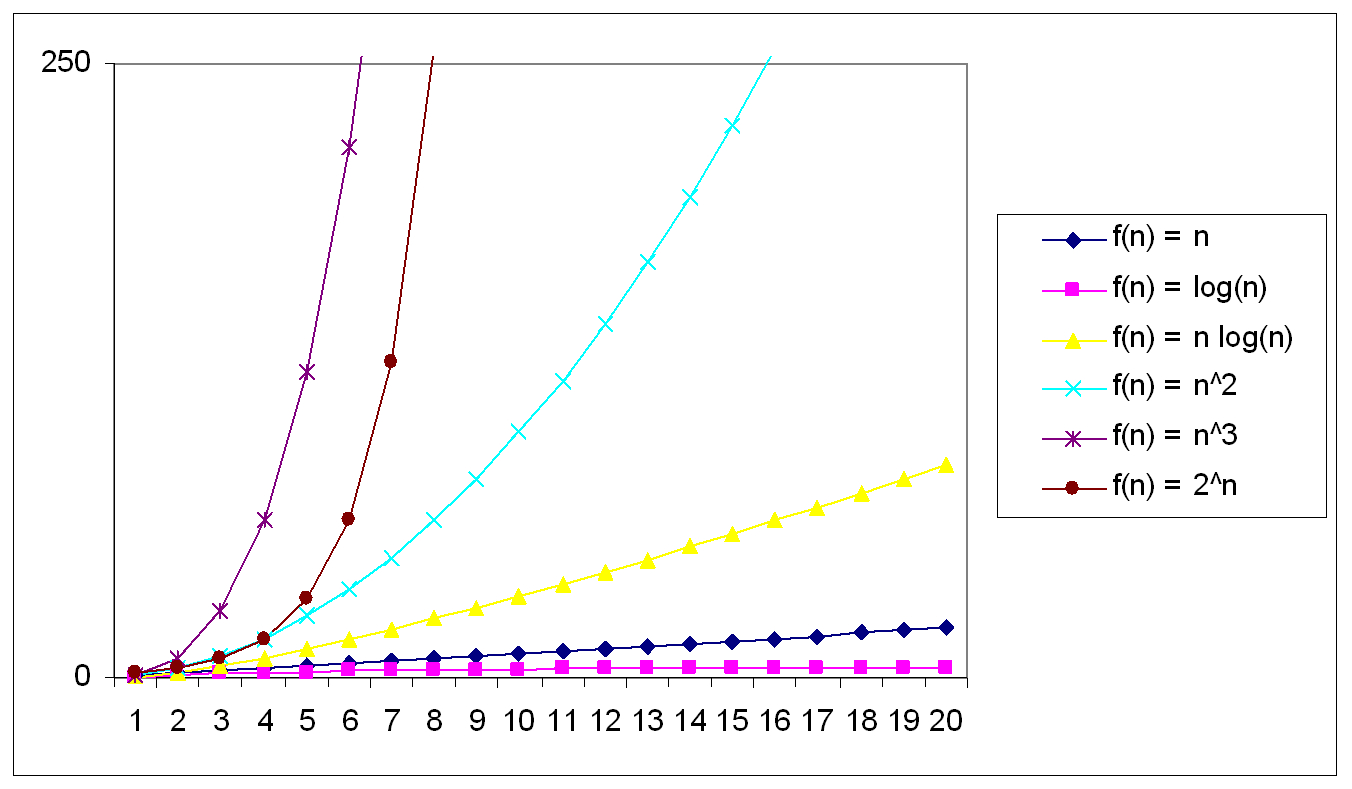
\includegraphics[height=0.95\textheight]{graph-1}
\end{frame}
\begin{frame}{}
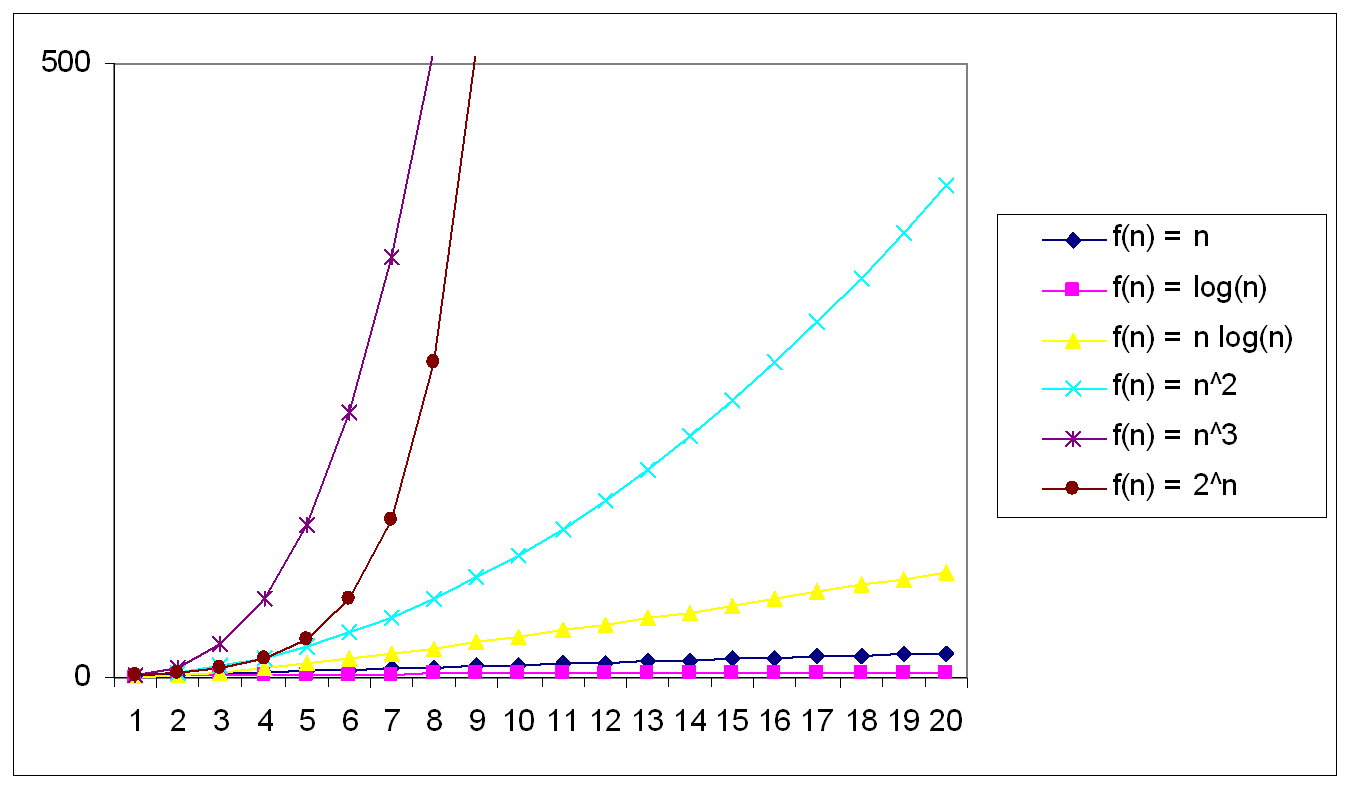
\includegraphics[height=0.95\textheight]{graph-2}
\end{frame}
\begin{frame}{}
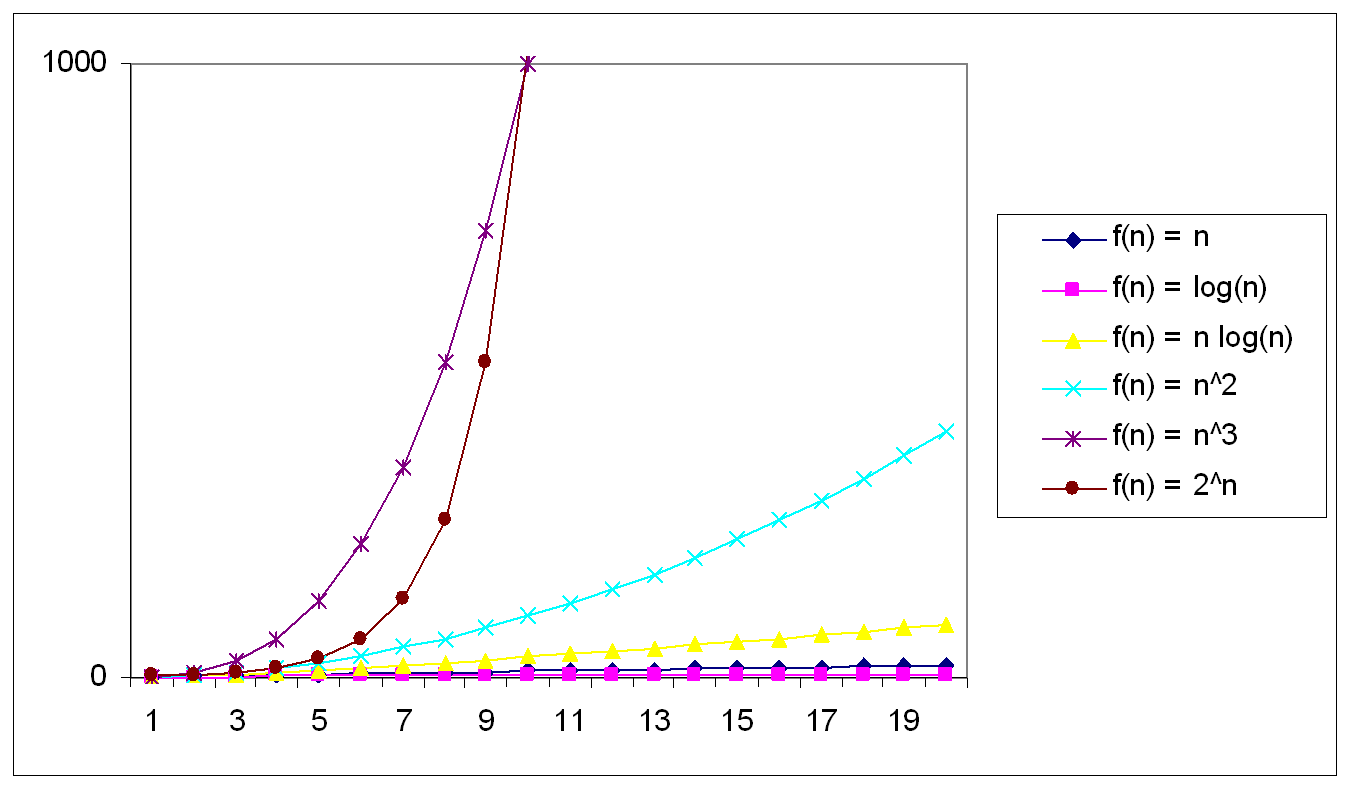
\includegraphics[height=0.95\textheight]{graph-3}
\end{frame}
\begin{frame}{}
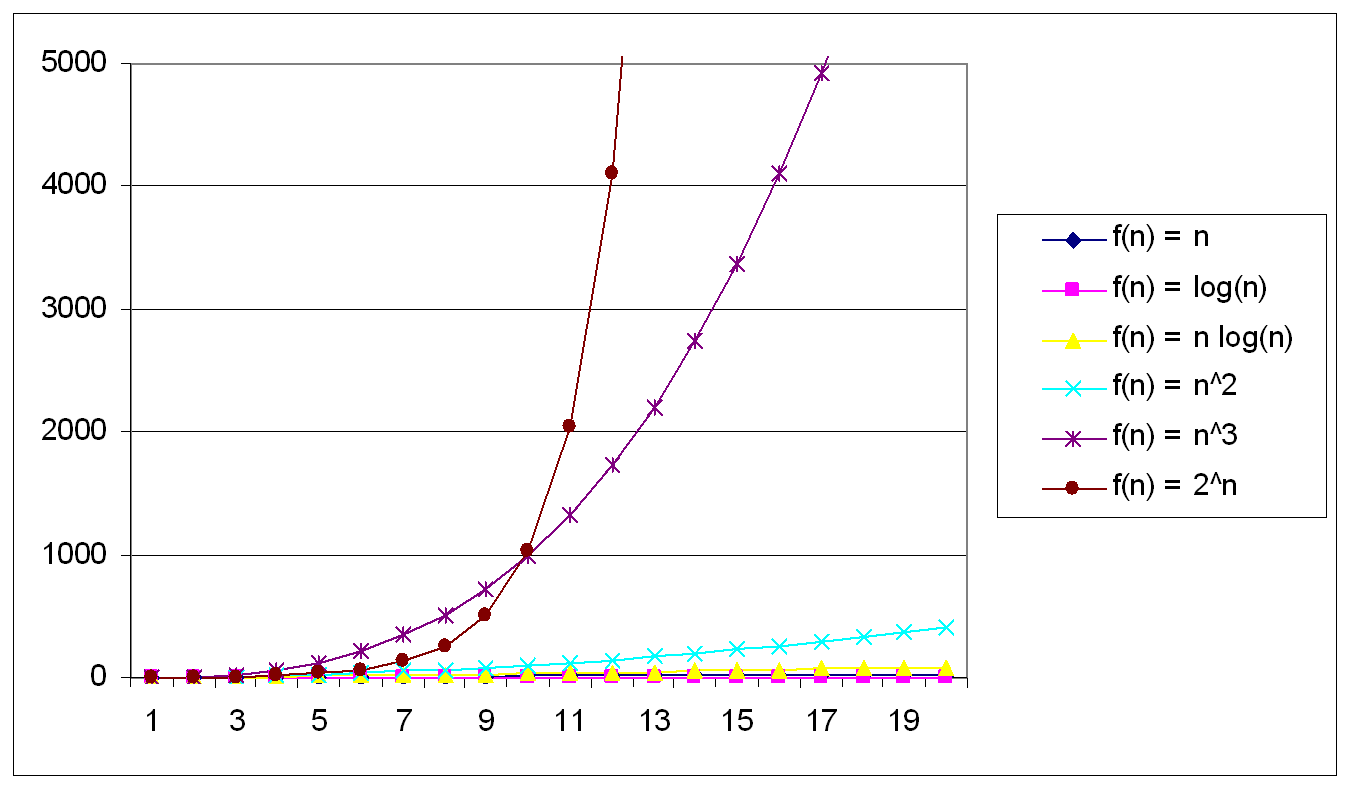
\includegraphics[height=0.95\textheight]{graph-4}
\end{frame}
\begin{frame}{}
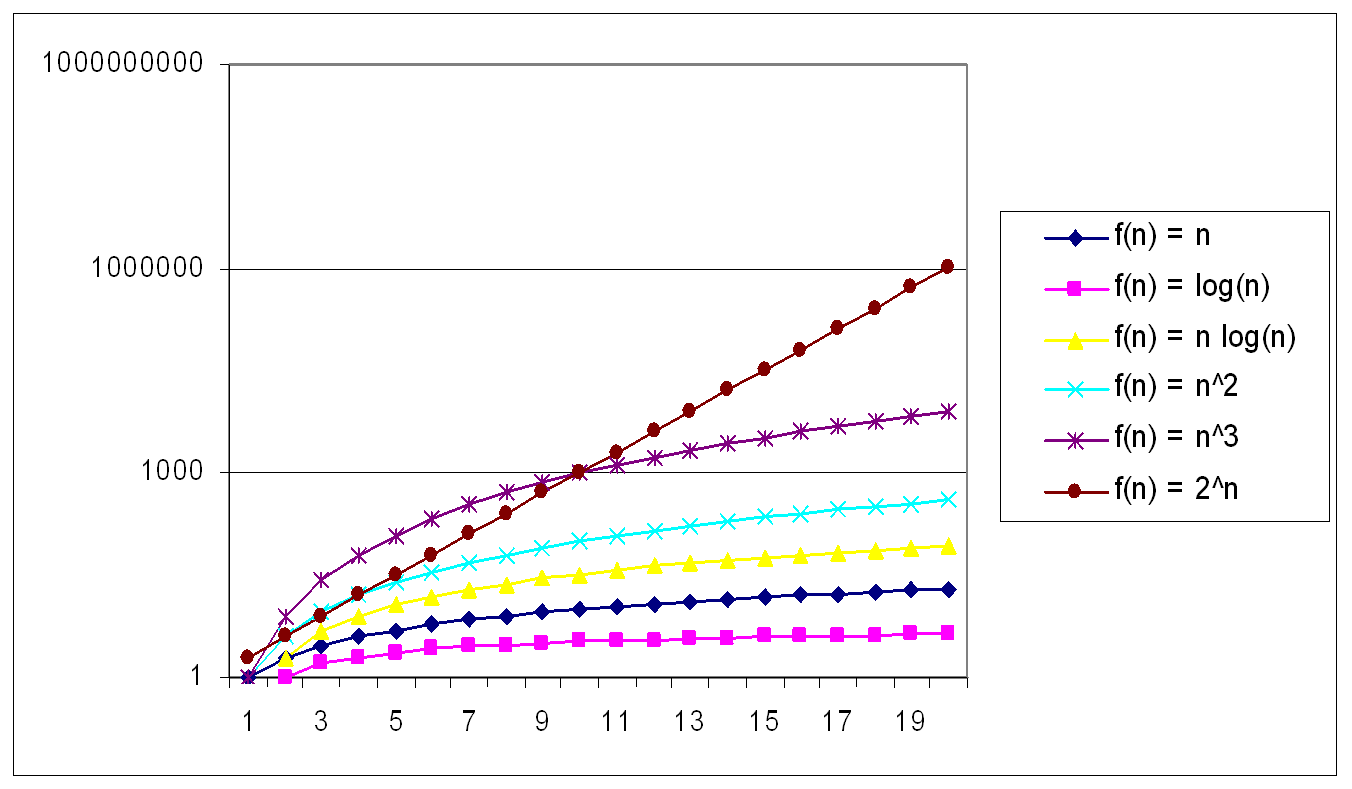
\includegraphics[height=0.95\textheight]{graph-5}
\end{frame}


% rules for calculating
    % for loops
    % nested loops --- inside out
    % if/else
\begin{frame}[fragile,label=thumb1]{big-oh rules of thumb (1)}
\lstset{
    language=C++,
    style=small
}
\begin{tikzpicture}
\tikzset{
    codeBox/.style={
        draw,thick
    },
    rt/.style={font=\small},
}
\node[codeBox] (forSimple) {
\begin{lstlisting}
for (int i = 0; i < N; ++i)
    foo();
\end{lstlisting}
};
\node[rt,right=1cm of forSimple] {$\text{runtime} = N \times (\text{runtime of \tt foo})$};

\node[codeBox,below=1cm of forSimple] (nestedForSimple) {
\begin{lstlisting}
for (int i = 0; i < N; ++i)
    for (int j = 0; j < M; ++j)
        foo();
\end{lstlisting}
};
\node[rt,right=1cm of nestedForSimple] {$\text{runtime} = N \times (M \times \text{runtime of \tt foo})$};

\node[codeBox,below=1cm of nestedForSimple] (nestedForHard) {
\begin{lstlisting}
for (int i = 0; i < N; ++i)
    for (int j = 0; j < i; ++j)
        foo();
\end{lstlisting}
};
\node[rt,right=1cm of nestedForHard] {$\text{runtime} = \sum_i^N j \times \text{runtime of \tt foo} = \Theta(N^2 \cdot \text{runtime of \tt foo})$};
\end{tikzpicture}
\end{frame}


% more examples of hierarchy (merge with earlier?)
\begin{frame}{$\Theta(1)$: constant time}
    \begin{itemize}
    \item constant time ($\Theta(1)$ time) --- runtime does not depend on input
    \vspace{.5cm}
    \item accessing an array element
    \item linked list insert/delete (at known end)
    \item getting a vector's size
    \item \ldots
    \end{itemize}
\end{frame}

\begin{frame}{is that really constant time}
    \begin{itemize}
    \item is getting vector's size really constant time?
    \item vector stores its size, but, for, e.g. $N=2^{10000}$, the size itself is \myemph{huge}
    \item our \textit{usual} assumption:
        \begin{itemize}
        \item treat ``sensible'' integer arithmetic as constant time
        \item (anything we'd keep in a {\tt long} or smaller variable in practice?)
        \end{itemize}
    \item can do other analysis, but uncommon
        \begin{itemize}
        \item e.g. ``bit complexity'' --- number of single bit operations
        \end{itemize}
    \end{itemize}
\end{frame}

\begin{frame}{$\Theta(\log n)$: logarithmic time}
    \begin{itemize}
    \item binary search of sorted array
        \begin{itemize}
        \item search space cut in half each iteration --- $\left\lceil\log_2 N\right\rceil$ iterations
        \end{itemize}
    \item \textit{balanced} tree search/insert
        \begin{itemize}
        \item height of tree (somehow) gaurenteed to be $\Theta(\log N)$
        \end{itemize}
    \end{itemize}
\end{frame}

\begin{frame}{$\Theta(n)$: linear}
    \begin{itemize}
        \item constant \# operations/element
            \vspace{.5cm}
        \item printing a list
        \item search in unsorted array
        \item search in linked list
        \item doubling the size of a vector
        \item \textit{unbalanced} binary search tree find/insert
    \end{itemize}
\end{frame}

\begin{frame}{$\Theta(n \log n)$: log-linear}
    \begin{itemize}
        \item fast comparison-based sorting 
            \begin{itemize}
            \item merge sort, heap sort, \ldots
            \end{itemize}
        \item quicksort \textit{if pivot choices are good}
        \item inserting $n$ elements into a balanced tree
    \end{itemize}
\end{frame}

\begin{frame}{$\Theta(n^2)$: quadratic}
    \begin{itemize}
        \item slow comparison-based sorting
            \begin{itemize}
            \item insertion sort, bubble sort, selection sort, \ldots
            \end{itemize}
        \item quicksort \textit{if pivot choices are bad}
        \item most doubly nested for loops that go up to $n$
    \end{itemize}
\end{frame}

\begin{frame}{$\Theta(2^{n^c})$, $c\ge1$: exponential}
    \begin{itemize}
        \item $n$-bit solution; try every $2^n$ of the possiblities
            \vspace{.5cm}
        \item crack a combination lock by trying every possiblity
        \item finding the best move in an $N\times N$ Go game (with Japanese rules)
        \item checking satisfiablity of Boolean expression*
        \item the Traveling Salesman problem*
        \item {\scriptsize *known algorithms --- maybe can do better?}
    \end{itemize}
\end{frame}

\begin{frame}{more?}
    \begin{itemize}
    \item $\Theta(n^3)$ --- find shortest paths between all pairs of $n$ nodes on a fully-connected graph
    \item approx. order $2^{n^{1/3}}$ --- best known integer factorization algorithm
    \end{itemize}
\end{frame}


% ----
% "determining running times"


